\documentclass[12pt,a4paper,english,twoside]{book}
\usepackage[german,english]{babel}
\usepackage[T1]{fontenc} 
\usepackage{amsfonts}
\usepackage{amsmath}
\usepackage{latexsym}
\usepackage{amssymb}
\usepackage{epsfig}
\usepackage{moreverb}
\usepackage{rotating}
\usepackage{enumerate}
\usepackage{graphics, graphicx,wrapfig}
\usepackage{fancybox}
\usepackage{picinpar,varioref,floatflt}
\usepackage{ae}
\usepackage{longtable}
\usepackage{textcomp}
\usepackage{float}
\usepackage{url}
\usepackage{unizhdt}
\usepackage{listings}
\usepackage{color}
\usepackage[backend=biber, sorting=none]{biblatex}

%%%%%%%%%%%%%%%%%%%%%%%%%%%%%%%%%%%%%%%%%%%%%%%%%%

% Define the language of the diploma thesis
\selectlanguage{english}
%\selectlanguage{german}

\pagestyle{headings}

\addbibresource{citations.bib}

\begin{document}

%%%%%%%%%%%%%%%%%%%%%%%%%%%%%%%%%%%%%%%%%%%%%%%%%%

% Define the author printed on the cover page
\author{Jonathan Burger}
% Define the city and country of the author
\authorcity{Zurich, Switzerland}
% Define the student ID (Matrikelnummer)
\studentid{13-746-698}
% Define the title with optional subtitle
\title{Collaborative DDoS Mitigation Based on Blockchains}
% Define the supervisors
\supervisors{Sina Rafati, Thomas Bocek}
% Define the submission date
\submissiondate{TBD}

%%%%%%%%%%%%%%%%%%%%%%%%%%%%%%%%%%%%%%%%%%%%%%%%%%

% Make the title page
\maketitle

% Make the imprint on the back of the cover page
\makeimprint

\pagenumbering{roman}

% Include the files of the diploma thesis
%\cleardoublepage

\chapter*{Abstract}
\addcontentsline{toc}{chapter}{Abstract}

\selectlanguage{german}

Attacken wie Distributed Denial-of-Service (DDoS) stellen ein immer gr{"o}sser werdende Gefahr dar f{"u}r Computernetzwerke und Internet-Services.
Existierende Strategien zur Bek{"a}mpfung von DDoS-Attacken sind ineffizient aufgrund mangelnder Ressourcen und Inflexibilit{"a}t.
Blockchains wie Ethereum erm{"o}glichen neue Methoden zur Mitigation von DDoS-Attacken. Mittels Smart Contract k{"o}nnen IP-Addressen von Attackierern auf einer dezentralisierten Plattform signalisiert werden, ohne zus{"a}tzliche Infrastruktur einzusetzen.
Diese Arbeit dokumentiert die Entwicklung mehrerer Smart Contracts zur Signalisierung von DDoS-Attacken und vergleicht sie, bespricht die Ethereum-Umgebung und ihre Auswirkungen auf die Architektur, gibt Auskunft {"u}ber Leistung sowie Kosten und evaluiert die Machbarkeit und Wirksamkeit einer blockchainbasierten L{"o}sung zur Bek{"a}mpfung von DDoS-Attacken.

\selectlanguage{english}

%\cleardoublepage
%\chapter*{Acknowledgments}
\addcontentsline{toc}{chapter}{Acknowledgments}

I would like to thank my supervisors, Thomas Bocek and Sina Rafati, for helping me find this topic and continually guiding me during this work with ideas and knowledge and even helping me with formal language.

I would also like to thank the other members of the Communication Systems Group doing research on blockchains who have provided me with their input as well.

Finally, I would like to thank Prof. Burkhard Stiller for making it possible to write my bachelor thesis at the Communication Systems Group and for providing feedback as well.


\tableofcontents

\cleardoublepage
\pagenumbering{arabic}
\chapter{Note about this intermediate report}

This is a work-in-progress version of my bachelor thesis.
I plan on continuing the thesis according to the task description and the previously worked out schedule.

The thesis is accompanied by code, always available under

https://github.com/JonnyBurger/ddos-bachelor-thesis.

For that access, an invitation is required until the thesis is finalized, but a copy from Thursday, June 1st is provided.

\chapter{Introduction}

\section{Blockchains and Ethereum}

A Blockchain is a decentralized database consisting of a chain of cryptographically secured units, called 'blocks'. Each block references the previous block and cannot be modified without breaking the subsequent blocks. A blockchain is continuously growing, as new data is inserted at the end of the chain.
The most popular application for blockchains are digital crypto currencies, the most widely used implementation is Bitcoin. With Bitcoin, which had it's breakthrough in 2008, network users can exchange tokens securely over a completely decentralized protocol. Because of this usefulness, these tokens are valued with real money, the total market capitalization of Bitcoin is several dozen millions.
 
Ethereum \cite{Ethereum} is blockchain protocol that is inspired by Bitcoin, but not only allows for sending and receiving of tokens, but also offers a scripting language called Solidity, which allows anyone to write programs which can be run on the blockchain. Examples for applications that could run on Ethereum are games like Tic-Tac-Toe or Poker, finance applications like venture capital funds and Initial Coin Offerings (a company raising funds by selling shares of it to investors).
An application is also called a smart contract and allows for storage of arbitrary information and allows for users to send transactions that mutate the storage. The creator of the smart contract controls with code the permissions of the users, the conditions and behaviors of the mutations. This enables a wide variety of possible applications, including a collaborative DDoS mitigation solution, which this thesis is about.

\section{Denial of Service and DDoS}

A Denial of Service (DoS) is when a machine or network resource that should be online is being disrupted. An attacker can either force a DoS by crafting a request payload causing a lot of computational work on the target machine or by flooding the target with requests. The motivation behind a DoS attack is that the attacker sees benefit in the victim's service being disrupted, be that disagreement with the service offered (activist attack), that the service is from a competitor, or that taking down a service brings pleasure to the victim.

A Distributed Denial of Service (DDoS) attack is a DoS attack where the requests are coming from many different sources. By distributing the requests, a denial of service attack can reach much higher magnitudes in terms of traffic and can become much harder to control.
Usually, an attacker takes control of as many internet-connected devices as possible by spreading malware, and then directing these devices to attack the victim.


\section{Motivation}

The amount of DDoS attacks globally is on the rise \cite{DDoSRise} and mitigation is happening only with limited success. 
DDoS protection is a burden for most services and requires human and financial resources. A standard tool for signaling DDoS attacks that can be used collaboratively would lower the investment needed to prepare for DDoS attacks.
The Ethereum blockchain is a database that is already available and that can not be taken down. With Solidity, the blockchain is scriptable and interfaces for storing and retrieving IP addresses can be programmed. With Ethereum being an readily available infrastructure independent from web services, it opens up an opportunity for storing signals of IP addresses.

\section{Description of Work}

The paper {"}A Blockchain-based Architecture for Collaborative DDoS Mitigation with Smart Contracts and SDN{"} \cite{OriginalPaper} proposes to use the Ethereum blockchain as a registry for IP addresses from which attacks are originating from. The data can then be read by ISPs who can filter out the malicious packets before they even reach the victim of the attack. This eliminates the need for additional architecture.

Three variants of a smart contract will be developed and compared to each other. Each smart contract serves the same purpose, the storage of a list of IP addresses. All variants accept the input of IP addresses and allow to read from it, although in different ways.
Our main objective is to eliminate the need to set up and maintain a database for this purpose.

The three variants are: 1. A smart contract that stores a list of all IP addresses on the blockchain, similar to the contract shown in the original paper \cite{OriginalPaper} (Listing 1-3). 2. A contract that points to a web resource containing the list of all IP addresses. 3. A contract that implements a bloom filter.

All contracts should support both whitelists and blacklists.
A whitelist, in this case, is a list of IP addresses that are explicitly allowed to access the server, while a blacklist is a list of IP addresses that are explicitly disallowed to access the service.
Both IPv4 and IPv6 addresses should be insertable. Furthermore, it should be made as easy as possible to modify the list. Additionally, the contract should make it possible to easily verify the identity of the reporter and prevent unauthorized modifications of entries on behalf of others. 

\section{Thesis Outline}

In Chapter 2, the characteristics of Ethereum smart contracts and their implications on our implementation are discussed, as well as the properties and mechanics of our solution and look at security risks.

In Chapter X, the smart contracts based on the planning in chapter 1 are being implemented. The chapter describes the implementation technique, testing strategy and documents the established protocols.

In Chapter 3, the developed smart contracts for cost and speed are benchmarked and compared. In addition, a generic cost model for smart contracts is being introduced and optimization possibilities are being explored.
In Chapter X, a recommendation is made for a smart contract variant and make a statement whether the developed approach based on our research is suitable for real-world use.

\chapter{Related Work}

This thesis aims to further explore the idea laid out by the paper "A Blockchain-based Architecture for Collaborative DDoS Mitigation with Smart Contracts and SDN" \cite{ThinkingAboutSmartContractSecurity}.

A proposal submitted to the Internet Engineering Task Force (IETF) \cite{IETFDraft} describes a protocol for signaling source IP addresses of DDoS attacks. 

\chapter{Development}

\section{Contract 1: Native storage}
The first variant that will be developed stores all IP addresses in the blockchain natively. The advantage is that all infrastructure is outsourced to the blockchain, making the solution completely decentralized. The disadvantage is that high gas fees make this the most costly solution and that the scale is limited in that the Ethereum blockchain is not designed to store data in the Gigabyte range.

\section{Contract 2: Pointer to web resource}
The second variant of the smart contract works around the space constraints and the big cost of the first variant by storing the list of IP addresses on a web resource and pointing to that on the blockchain. The advantage is that it works on a much larger scale. The disadvantage is that a web server needs to be set up and a separate standard has to be established describing the format of the web resource. This solution is also more prone to connectivity issues and does not take advantage of the decentralization and immutability of the blockchain.

\subsection{Web resource}
When we point to a web resource, we need to think about the design of the architecture that we have off the blockchain. By storing a URL in the blockchain, it is already implied that we plan to connect to the resource using HTTP(S), which is a suitable protocol for our needs. The format of the web resource we point to could be in any format imaginable. There are a few properties which are desirable: 1. Portability: To increase the adoption of our solution, use an already existing format like XML, CSV or JSON. 2. Upgradeability: The format should be able to be developed further in the future to enable more features, with backwards compatibility (which is hard if the format is CSV-like). 3. Streamability: As we expect these lists to become very large, it would be useful to design the format in a way that it can already be partially evaluated while not yet fully loaded. Downloading a resource can take quite some time and we would like to not have to load the full list into memory. This is easy with CSV, as the file can be read line by line, but hard with XML or JSON, which needs to be fully loaded in order to be valid.
This is a classic 'Pick two out of three'-scenario, as these properties are conflicting with each other.
Finally, we need to think about whether the web resource should be immutable or not. Immutable means that the content of the web page can never change. Additions or deletions to the list are not supported, if the list had to be updated, it would have to move to a different URL and the entry in the blockchain has to be updated as well. This is not only a bad thing, as otherwise the client who accesses the resource has to worry about checking for updates. A hash can be generated for an immutable file, which could be stored in the blockchain as well and allow the clients to validate that the list has not been altered since it was registered in the smart contract, which is more in the spirit of the blockchain. If an asset is immutable, it can be easily outsourced to a CDN, which are harder to take down using a DDoS attack.
In summary, immutability makes it slower (and potentially more expensive) to register changes, but has some advantages.

\section{Contract 3: Bloom filter}
The third variant of the smart contract is a standalone contract that solves the scalability issue by storing not the whole list of IP addresses but only limited information from which it can only be said with a likelihood whether an IP address was blocked. The bloom filter contract is a nice balance between leveraging the blockchain and using little space, however it gives up perfect accuracy.

\section{IPv6 support}

With IPv4 addresses being 32 bits long, only 232 combinations possible and the amount of free addresses is almost exhausted, which is the reason that we are currently in a transition phase from IPv4 to IPv6. Therefore it makes sense to support both formats. Two ways of supporting both IPv4 and IPv6 could be considered:

With IPv4 addresses being 32 bits long, only 232 combinations possible and the amount of free addresses is almost exhausted, which is the reason that we are currently in a transition phase from IPv4 to IPv6. Therefore it makes sense to support both formats. Two ways of supporting both IPv4 and IPv6 could be considered:
The first is to represent IPv4 addresses as IPv6 addresses. The most widespread format is defined in RFC 3493: 80 bits of zeros, 16 bits of ones and then the IPv4 address. So for example the IPv4 address \texttt{46.101.96.149} would be \texttt{0:0:0:0:0:ffff:2e65:6095} in IPv6 hex representation. In fact, this notation is supported by the Linux kernel and macOS natively, in a web browser \texttt{http://[::ffff:2e65:6095]} will display the same website as \texttt{http://46.101.96.149}.
The other option would be to use a flag indicating whether an address is IPv4 or IPv6. If mainly IPv4 addresses are stored in a contract, this would yield a space benefit.
Given that there is already a standardized solution for notating IPv4 in IPv6 format, we are proceeding with the first option.

\section{IP verification}
IP verification
In all variants of the smart contract, owners of destination IP addresses can store source IP addresses they want blocked in the smart contract. In order to establish trust, we are interested in automatically verifying the ownership of the destination IP addresses. This is a challenging task, as is explained in this section. Using certificates to validate IP ownerships in Solidity is currently not practical for at least two reasons.
It is a computationally expensive task that would require more gas than the gas limit allows and there is no implementation of certificate verification in Solidity. Certificate verification, as it is most commonly done with OpenSSL, would have to be ported ported to Solidity, which is complex.
There is however a proposal to add certificate validation on a language-level (Ethereum Improvement Proposal \#74). As of writing, it looks like the intent is to add BigInt to the Ethereum Virtual Machine, which could enable certificate validation.
Since everything in the blockchain is public including stored certificates and IP addresses, it is not required that certificates are validated in Solidity, it can be done off the blockchain.
The second challenge is obtaining a certificate. As there is no way to mathematically or logically prove that somebody is the owner of an IP (it can be spoofed), the certificate process of domains could be applied to IPs: There are certificate authority (CA) whose business is to provide a service validating the ownership of a domain. These CAs need to make investments in establishing a system that securely validates a domain and manages the certificates that are issued. Only if a CA has high standards their certificates are trustworthy. That is why nearly all CAs for domains issue certificates for a fee or need to generate revenue by sponsorships. Although it is technically possible to issue a SSL certificate for an IP address, it is very uncommon. GlobalSign\footnote{https://support.globalsign.com/customer/portal/articles/1216536-securing-a-public-ip-address---ssl-certificates} is the only provider known to us that does this, and requires that the IP is registered in the RIPE database.
A system that currently exists for domain could be introduced by the industry for IP addresses, but is very complicated and defeats the purpose of using the blockchain as the original idea was to remove the need for additional infrastructure.

\section{Validating Smart contracts during development}
Developing a smart contract requires a compiler and a blockchain on which the developer can test whether the smart contract behaves as desired. A compiler, such as solc, will warn about syntax errors and does not compile invalid Solidity code, indicating to the developer that there is an error in the code. While compilers provide a first layer of assurance by only compiling valid contracts with valid syntax, it is still possible to write code with behavioral bugs and security vulnerabilities. As with any software, developers need a workflow which allows them to test their changes fast and efficiently. The main ethereum blockchain is unsuitable for validating the correctness of the code manually. There are significant costs to deploy a contract to the blockchain, also it requires some time to receive the confirmations. It is also frowned upon to use the main blockchain for testing purposes, as all network participants need to download all blocks. This is not the case in the testnet, which is a seperate blockchain for testing purposes. Even better, there is a test framework called TestRPC that makes it possible to set up a local blockchain for testing. Using TestRPC, it is possible to simulate deployments and transactions of smart contracts with no confirmation delay. Out of the box, TestRPC sets up multiple ethereum accounts, so it easy to switch the message sender address and test whether the security features of the developed smart contract are working as desired. This makes TestRPC the ideal blockchain for developing.
In addition to manual testing, the robustness should be validated by unit tests, just like in any other piece of software. This allows to automatically validate that all assertions are still true when a change is introduced to the contract. A robust contract should have unit tests validating that normal use of the contract features result in correct behaviour, as well as edge cases and abuse of the contract features handled correctly. Examples of that are: Calling a function without permission, calling a function more often than expected, calling a function with unexpected arguments, such as null arguments, wrong types or a big payload.
I have used TestRPC, the Javascript "solc" compiler, and the "ava" testing framework to set up a test environment. Each test is completely atomic and independent from other ones, that means that for each test, a separate TestRPC blockchain is created and the scenario is run on it. After the test is finished, the blockchain and the accounts get destroyed. This complete isolation of each test is good practice, as side-effects can be ruled out. With "ava", the tests can be run in parallel, making it faster to run the whole test suite. However, there are many other generic test frameworks that work as well and have their own advantages and disadvantages. One interesting framework is Truffle\footnote{http://truffleframework.com/}, which provides helpers for developing and testing Solidity contracts. Truffle tries to make the process described in this section easier and looks very promising, but is still in beta. For the reason that the framework is still very much in development and changing, and that I have only discovered it after already having a solution working, I did not use it.
For real-world smart contract applications, testing is not enough, critical contracts should be audited by computer security professionals before being deployed. As the aim of this thesis is to document a proof-of-concept DDoS mitigation application, no audit will be conducted.

\section{Security considerations with Solidity}
Code vulnerabilities are more common in Ethereum than in other environments. The whole blockchain data is public, and serious contracts are made open source in order to create trust for the people who use it. Therefore applications are auditable and bugs are more likely to be found.The application must also regulate itself and can in most cases not recover from an attack.
In addition to that, the language Solidity aims to have a syntax similar to JavaScript and is therefore quite loose with enforcing the correct type. Static code analysis tools (such as Solium) are also not yet up to par with other languages.
In this section, we will explore some common "traps" that can lead to security exploits, partially taken from a list compiled by the co-founder of Ethereum \cite{ThinkingAboutSmartContractSecurity}.

\subsection{Constructor naming exploit}
Simple human mistakes can lead to the contract being vulnerable. The 'Rubixi' contract has a different constructor name than contract name. Therefore the constructor does not get called on deployment, but can be called as a transaction. If done so, the caller of the transaction becomes the owner of the contract. Because of more unfortunate design of the contract, the bug became not immediately apparent and the Solidity contract was correct.

\definecolor{dkgreen}{rgb}{0,0.6,0}
\definecolor{gray}{rgb}{0.5,0.5,0.5}
\definecolor{mauve}{rgb}{0.58,0,0.82}

\lstset{frame=tb,
  language=Java,
  aboveskip=3mm,
  belowskip=3mm,
  showstringspaces=false,
  columns=flexible,
  basicstyle={\small\ttfamily},
  numbers=none,
  numberstyle=\tiny\color{gray},
  keywordstyle=\color{blue},
  commentstyle=\color{dkgreen},
  stringstyle=\color{mauve},
  breaklines=true,
  breakatwhitespace=true,
  tabsize=3
}

\lstinputlisting{snippets/rubixi.sol}


\subsection{Public data}
A misconception is that stored data can be made private on the blockchain. A rock-paper-scissor contract which people used for gambling turned out to have a trivial flaw where the first move could be seen - rock would have the value \texttt{0x60689557} and scissor and paper have a different one.
The main takeaway is that in our case, the stored IP addresses will be public (although maybe obfuscated) to everybody. Even attackers can determine the list of IPs that are blocked. The contract should be created in a way that minifies the usefulness for attackers, for example the pattern of the IPs should not make the way how IPs are being blocked predictable.

\subsection{Loops}
The section "Security Considerations" of the Solidity documentation warns about loops that have a non-fixed amount of iterations. With a high number of iterations, the block gas limit could be reached and according to the Solidity documentations "cause the complete contract to be stalled at a certain point". In the reference contract, the function blockIPv4() has a loop whose amount of iterations are dependant of a transaction argument. The contract has to be tested with a big payload and a solution needs to be developed.
Furthermore, even for constant functions (which are executed locally and have no gas limit), there can be bugs. If, in the reference contract there would be a slight change:

\lstdefinelanguage{diff}{
  morecomment=[f][\color{blue}]{@@},     % group identifier
  morecomment=[f][\color{red}]-,         % deleted lines 
  morecomment=[f][\color{green}]+,       % added lines
  morecomment=[f][\color{magenta}]{---}, % Diff header lines (must appear after +,-)
  morecomment=[f][\color{magenta}]{+++},
}

\lstset{frame=tb,
  language=diff,
  aboveskip=3mm,
  belowskip=3mm,
  showstringspaces=false,
  columns=flexible,
  basicstyle={\small\ttfamily},
  numbers=none,
  numberstyle=\tiny\color{gray},
  keywordstyle=\color{blue},
  commentstyle=\color{dkgreen},
  stringstyle=\color{mauve},
  breaklines=true,
  breakatwhitespace=true,
  tabsize=3
}

\lstinputlisting{snippets/loop-bug.diff}


We would introduce a bug. \texttt{var} would be interpreted as \texttt{uint8}, and if there are more than 255 entries in the \texttt{drop\_src\_ipv4} array, there would be an overflow leading to an infinite loop.
This bug can be simply avoided by disallowing \texttt{var} in the code or by being aware of the issue.


\subsection{Re-Entry bugs using .call()}

The \texttt{.call()} method in Solidity is dangerous as it can execute code from external contracts. This weakness was first exploited in the DAO smart contract, which had over 50 million USD stored in it. The main takeaway from this incident is that \texttt{.call()} can call any public function, even the function from which it was called from, leading to recursion.
The following example is not safe:

\definecolor{dkgreen}{rgb}{0,0.6,0}
\definecolor{gray}{rgb}{0.5,0.5,0.5}
\definecolor{mauve}{rgb}{0.58,0,0.82}

\lstset{frame=tb,
  language=Java,
  aboveskip=3mm,
  belowskip=3mm,
  showstringspaces=false,
  columns=flexible,
  basicstyle={\small\ttfamily},
  numbers=none,
  numberstyle=\tiny\color{gray},
  keywordstyle=\color{blue},
  commentstyle=\color{dkgreen},
  stringstyle=\color{mauve},
  breaklines=true,
  breakatwhitespace=true,
  tabsize=3
}

\lstinputlisting{snippets/reentry-bug.sol}


Let's say that the balance of an account is 10 and that account calls the withdraw method. The account can execute arbitrary code when \texttt{msg.sender.call()} is called on line 3, so \texttt{withdraw()} can also be called again before line 4 of the above snippet is reached. An attacker could withdraw more than what its balance is. The vulnerability could be mitigated by using \texttt{.send()} instead of \texttt{.call()} in the example above.

\subsection{Call stack depth attack}

The call stack depth gets increased when a function calls another function, and if a function returns, the call stack depth gets decreased. A long call stack can be produced by excessive recursion. Solidity has a 1024 call stack depth limit - this means that Solidity could for example not compute the 1025th fibonacci number using recursion.
The deterministic depth limit of Solidity proves to be an attack vector. An attacker could craft a function that calls itself 1023 times and on the 1024th time calls another, vulnerable function, that stops execution as soon as a subfunction is called, because the maximum call stack size is reached. An attacker might force a function to only partially execute, which is a problem, if for example a withdraw function is composited of a subfunction that sends funds and a function that decreases the users balance.
The core development team of Ethereum wants to solve this problem on a language-level in EIP \#150 soon, therefore it will not be further discussed here.

\chapter{Development}

\section{Contract 1: Native storage}
The first variant that will be developed stores all IP addresses in the blockchain natively. The advantage is that all infrastructure is outsourced to the blockchain, making the solution completely decentralized. The disadvantage is that high gas fees make this the most costly solution and that the scale is limited in that the Ethereum blockchain is not designed to store data in the Gigabyte range.

\section{Contract 2: Pointer to web resource}
The second variant of the smart contract works around the space constraints and the big cost of the first variant by storing the list of IP addresses on a web resource and pointing to that on the blockchain. The advantage is that it works on a much larger scale. The disadvantage is that a web server needs to be set up and a separate standard has to be established describing the format of the web resource. This solution is also more prone to connectivity issues and does not take advantage of the decentralization and immutability of the blockchain.

\subsection{Web resource}
When we point to a web resource, we need to think about the design of the architecture that we have off the blockchain. By storing a URL in the blockchain, it is already implied that we plan to connect to the resource using HTTP(S), which is a suitable protocol for our needs. The format of the web resource we point to could be in any format imaginable. There are a few properties which are desirable: 1. Portability: To increase the adoption of our solution, use an already existing format like XML, CSV or JSON. 2. Upgradeability: The format should be able to be developed further in the future to enable more features, with backwards compatibility (which is hard if the format is CSV-like). 3. Streamability: As we expect these lists to become very large, it would be useful to design the format in a way that it can already be partially evaluated while not yet fully loaded. Downloading a resource can take quite some time and we would like to not have to load the full list into memory. This is easy with CSV, as the file can be read line by line, but hard with XML or JSON, which needs to be fully loaded in order to be valid.
This is a classic 'Pick two out of three'-scenario, as these properties are conflicting with each other.
Finally, we need to think about whether the web resource should be immutable or not. Immutable means that the content of the web page can never change. Additions or deletions to the list are not supported, if the list had to be updated, it would have to move to a different URL and the entry in the blockchain has to be updated as well. This is not only a bad thing, as otherwise the client who accesses the resource has to worry about checking for updates. A hash can be generated for an immutable file, which could be stored in the blockchain as well and allow the clients to validate that the list has not been altered since it was registered in the smart contract, which is more in the spirit of the blockchain. If an asset is immutable, it can be easily outsourced to a CDN, which are harder to take down using a DDoS attack.
In summary, immutability makes it slower (and potentially more expensive) to register changes, but has some advantages.

\section{Contract 3: Bloom filter}
The third variant of the smart contract is a standalone contract that solves the scalability issue by storing not the whole list of IP addresses but only limited information from which it can only be said with a likelihood whether an IP address was blocked. The bloom filter contract is a nice balance between leveraging the blockchain and using little space, however it gives up perfect accuracy.

\section{IPv6 support}

With IPv4 addresses being 32 bits long, only 232 combinations possible and the amount of free addresses is almost exhausted, which is the reason that we are currently in a transition phase from IPv4 to IPv6. Therefore it makes sense to support both formats. Two ways of supporting both IPv4 and IPv6 could be considered:

With IPv4 addresses being 32 bits long, only 232 combinations possible and the amount of free addresses is almost exhausted, which is the reason that we are currently in a transition phase from IPv4 to IPv6. Therefore it makes sense to support both formats. Two ways of supporting both IPv4 and IPv6 could be considered:
The first is to represent IPv4 addresses as IPv6 addresses. The most widespread format is defined in RFC 3493: 80 bits of zeros, 16 bits of ones and then the IPv4 address. So for example the IPv4 address \texttt{46.101.96.149} would be \texttt{0:0:0:0:0:ffff:2e65:6095} in IPv6 hex representation. In fact, this notation is supported by the Linux kernel and macOS natively, in a web browser \texttt{http://[::ffff:2e65:6095]} will display the same website as \texttt{http://46.101.96.149}.
The other option would be to use a flag indicating whether an address is IPv4 or IPv6. If mainly IPv4 addresses are stored in a contract, this would yield a space benefit.
Given that there is already a standardized solution for notating IPv4 in IPv6 format, we are proceeding with the first option.

\section{IP verification}
IP verification
In all variants of the smart contract, owners of destination IP addresses can store source IP addresses they want blocked in the smart contract. In order to establish trust, we are interested in automatically verifying the ownership of the destination IP addresses. This is a challenging task, as is explained in this section. Using certificates to validate IP ownerships in Solidity is currently not practical for at least two reasons.
It is a computationally expensive task that would require more gas than the gas limit allows and there is no implementation of certificate verification in Solidity. Certificate verification, as it is most commonly done with OpenSSL, would have to be ported ported to Solidity, which is complex.
There is however a proposal to add certificate validation on a language-level (Ethereum Improvement Proposal \#74). As of writing, it looks like the intent is to add BigInt to the Ethereum Virtual Machine, which could enable certificate validation.
Since everything in the blockchain is public including stored certificates and IP addresses, it is not required that certificates are validated in Solidity, it can be done off the blockchain.
The second challenge is obtaining a certificate. As there is no way to mathematically or logically prove that somebody is the owner of an IP (it can be spoofed), the certificate process of domains could be applied to IPs: There are certificate authority (CA) whose business is to provide a service validating the ownership of a domain. These CAs need to make investments in establishing a system that securely validates a domain and manages the certificates that are issued. Only if a CA has high standards their certificates are trustworthy. That is why nearly all CAs for domains issue certificates for a fee or need to generate revenue by sponsorships. Although it is technically possible to issue a SSL certificate for an IP address, it is very uncommon. GlobalSign\footnote{https://support.globalsign.com/customer/portal/articles/1216536-securing-a-public-ip-address---ssl-certificates} is the only provider known to us that does this, and requires that the IP is registered in the RIPE database.
A system that currently exists for domain could be introduced by the industry for IP addresses, but is very complicated and defeats the purpose of using the blockchain as the original idea was to remove the need for additional infrastructure.

\section{Validating Smart contracts during development}
Developing a smart contract requires a compiler and a blockchain on which the developer can test whether the smart contract behaves as desired. A compiler, such as solc, will warn about syntax errors and does not compile invalid Solidity code, indicating to the developer that there is an error in the code. While compilers provide a first layer of assurance by only compiling valid contracts with valid syntax, it is still possible to write code with behavioral bugs and security vulnerabilities. As with any software, developers need a workflow which allows them to test their changes fast and efficiently. The main ethereum blockchain is unsuitable for validating the correctness of the code manually. There are significant costs to deploy a contract to the blockchain, also it requires some time to receive the confirmations. It is also frowned upon to use the main blockchain for testing purposes, as all network participants need to download all blocks. This is not the case in the testnet, which is a seperate blockchain for testing purposes. Even better, there is a test framework called TestRPC that makes it possible to set up a local blockchain for testing. Using TestRPC, it is possible to simulate deployments and transactions of smart contracts with no confirmation delay. Out of the box, TestRPC sets up multiple ethereum accounts, so it easy to switch the message sender address and test whether the security features of the developed smart contract are working as desired. This makes TestRPC the ideal blockchain for developing.
In addition to manual testing, the robustness should be validated by unit tests, just like in any other piece of software. This allows to automatically validate that all assertions are still true when a change is introduced to the contract. A robust contract should have unit tests validating that normal use of the contract features result in correct behaviour, as well as edge cases and abuse of the contract features handled correctly. Examples of that are: Calling a function without permission, calling a function more often than expected, calling a function with unexpected arguments, such as null arguments, wrong types or a big payload.
I have used TestRPC, the Javascript "solc" compiler, and the "ava" testing framework to set up a test environment. Each test is completely atomic and independent from other ones, that means that for each test, a separate TestRPC blockchain is created and the scenario is run on it. After the test is finished, the blockchain and the accounts get destroyed. This complete isolation of each test is good practice, as side-effects can be ruled out. With "ava", the tests can be run in parallel, making it faster to run the whole test suite. However, there are many other generic test frameworks that work as well and have their own advantages and disadvantages. One interesting framework is Truffle\footnote{http://truffleframework.com/}, which provides helpers for developing and testing Solidity contracts. Truffle tries to make the process described in this section easier and looks very promising, but is still in beta. For the reason that the framework is still very much in development and changing, and that I have only discovered it after already having a solution working, I did not use it.
For real-world smart contract applications, testing is not enough, critical contracts should be audited by computer security professionals before being deployed. As the aim of this thesis is to document a proof-of-concept DDoS mitigation application, no audit will be conducted.

\section{Security considerations with Solidity}
Code vulnerabilities are more common in Ethereum than in other environments. The whole blockchain data is public, and serious contracts are made open source in order to create trust for the people who use it. Therefore applications are auditable and bugs are more likely to be found.The application must also regulate itself and can in most cases not recover from an attack.
In addition to that, the language Solidity aims to have a syntax similar to JavaScript and is therefore quite loose with enforcing the correct type. Static code analysis tools (such as Solium) are also not yet up to par with other languages.
In this section, we will explore some common "traps" that can lead to security exploits, partially taken from a list compiled by the co-founder of Ethereum \cite{ThinkingAboutSmartContractSecurity}.

\subsection{Constructor naming exploit}
Simple human mistakes can lead to the contract being vulnerable. The 'Rubixi' contract has a different constructor name than contract name. Therefore the constructor does not get called on deployment, but can be called as a transaction. If done so, the caller of the transaction becomes the owner of the contract. Because of more unfortunate design of the contract, the bug became not immediately apparent and the Solidity contract was correct.

\definecolor{dkgreen}{rgb}{0,0.6,0}
\definecolor{gray}{rgb}{0.5,0.5,0.5}
\definecolor{mauve}{rgb}{0.58,0,0.82}

\lstset{frame=tb,
  language=Java,
  aboveskip=3mm,
  belowskip=3mm,
  showstringspaces=false,
  columns=flexible,
  basicstyle={\small\ttfamily},
  numbers=none,
  numberstyle=\tiny\color{gray},
  keywordstyle=\color{blue},
  commentstyle=\color{dkgreen},
  stringstyle=\color{mauve},
  breaklines=true,
  breakatwhitespace=true,
  tabsize=3
}

\lstinputlisting{snippets/rubixi.sol}


\subsection{Public data}
A misconception is that stored data can be made private on the blockchain. A rock-paper-scissor contract which people used for gambling turned out to have a trivial flaw where the first move could be seen - rock would have the value \texttt{0x60689557} and scissor and paper have a different one.
The main takeaway is that in our case, the stored IP addresses will be public (although maybe obfuscated) to everybody. Even attackers can determine the list of IPs that are blocked. The contract should be created in a way that minifies the usefulness for attackers, for example the pattern of the IPs should not make the way how IPs are being blocked predictable.

\subsection{Loops}
The section "Security Considerations" of the Solidity documentation warns about loops that have a non-fixed amount of iterations. With a high number of iterations, the block gas limit could be reached and according to the Solidity documentations "cause the complete contract to be stalled at a certain point". In the reference contract, the function blockIPv4() has a loop whose amount of iterations are dependant of a transaction argument. The contract has to be tested with a big payload and a solution needs to be developed.
Furthermore, even for constant functions (which are executed locally and have no gas limit), there can be bugs. If, in the reference contract there would be a slight change:

\lstdefinelanguage{diff}{
  morecomment=[f][\color{blue}]{@@},     % group identifier
  morecomment=[f][\color{red}]-,         % deleted lines 
  morecomment=[f][\color{green}]+,       % added lines
  morecomment=[f][\color{magenta}]{---}, % Diff header lines (must appear after +,-)
  morecomment=[f][\color{magenta}]{+++},
}

\lstset{frame=tb,
  language=diff,
  aboveskip=3mm,
  belowskip=3mm,
  showstringspaces=false,
  columns=flexible,
  basicstyle={\small\ttfamily},
  numbers=none,
  numberstyle=\tiny\color{gray},
  keywordstyle=\color{blue},
  commentstyle=\color{dkgreen},
  stringstyle=\color{mauve},
  breaklines=true,
  breakatwhitespace=true,
  tabsize=3
}

\lstinputlisting{snippets/loop-bug.diff}


We would introduce a bug. \texttt{var} would be interpreted as \texttt{uint8}, and if there are more than 255 entries in the \texttt{drop\_src\_ipv4} array, there would be an overflow leading to an infinite loop.
This bug can be simply avoided by disallowing \texttt{var} in the code or by being aware of the issue.


\subsection{Re-Entry bugs using .call()}

The \texttt{.call()} method in Solidity is dangerous as it can execute code from external contracts. This weakness was first exploited in the DAO smart contract, which had over 50 million USD stored in it. The main takeaway from this incident is that \texttt{.call()} can call any public function, even the function from which it was called from, leading to recursion.
The following example is not safe:

\definecolor{dkgreen}{rgb}{0,0.6,0}
\definecolor{gray}{rgb}{0.5,0.5,0.5}
\definecolor{mauve}{rgb}{0.58,0,0.82}

\lstset{frame=tb,
  language=Java,
  aboveskip=3mm,
  belowskip=3mm,
  showstringspaces=false,
  columns=flexible,
  basicstyle={\small\ttfamily},
  numbers=none,
  numberstyle=\tiny\color{gray},
  keywordstyle=\color{blue},
  commentstyle=\color{dkgreen},
  stringstyle=\color{mauve},
  breaklines=true,
  breakatwhitespace=true,
  tabsize=3
}

\lstinputlisting{snippets/reentry-bug.sol}


Let's say that the balance of an account is 10 and that account calls the withdraw method. The account can execute arbitrary code when \texttt{msg.sender.call()} is called on line 3, so \texttt{withdraw()} can also be called again before line 4 of the above snippet is reached. An attacker could withdraw more than what its balance is. The vulnerability could be mitigated by using \texttt{.send()} instead of \texttt{.call()} in the example above.

\subsection{Call stack depth attack}

The call stack depth gets increased when a function calls another function, and if a function returns, the call stack depth gets decreased. A long call stack can be produced by excessive recursion. Solidity has a 1024 call stack depth limit - this means that Solidity could for example not compute the 1025th fibonacci number using recursion.
The deterministic depth limit of Solidity proves to be an attack vector. An attacker could craft a function that calls itself 1023 times and on the 1024th time calls another, vulnerable function, that stops execution as soon as a subfunction is called, because the maximum call stack size is reached. An attacker might force a function to only partially execute, which is a problem, if for example a withdraw function is composited of a subfunction that sends funds and a function that decreases the users balance.
The core development team of Ethereum wants to solve this problem on a language-level in EIP \#150 soon, therefore it will not be further discussed here.

\chapter{...}


\chapter{Evaluation}

\section{Cost Benchmark}

This section aims to provide a rough guidance on expected cost for each variant of the smart contract.

For calculating costs of Ethereum usage, the unit used is gas as it is mostly predictable. This is to make the numbers still usable in the future as gas price and Ether-to-USD conversion rate will experience variance over time.

For variant 1, a benchmark script was created\footnote{The source code can be found under \texttt{v1-gas-benchmark.js}. The benchmark can be executed with \texttt{node index v1-gas-benchmark}.}. The benchmark calculates the cumulative gas spent on contract creation and IP address insertion. Two cases were calculated: For the worst case, each IP address was inserted in a separate transaction. For the best case, reports were bundled into one transaction. The benchmark was executed in both cases for 1 IP address, then 2 IP addresses and so forth up to 20 IP addresses. The resulting costs are displayed in Figure \ref{fig:v1-gas-cost}.

\begin{figure}[H]
\centering
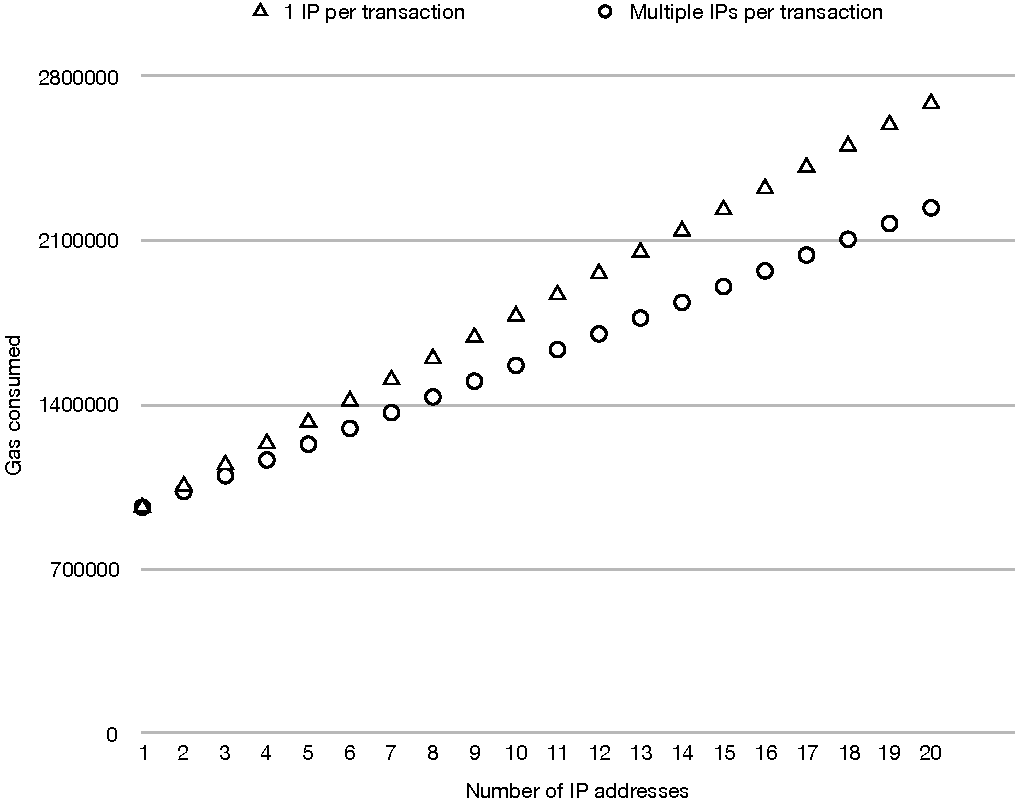
\includegraphics[width=0.7\textwidth]{v1-gas-cost.pdf}
\caption{Gas cost incurred using variant 1}
\label{fig:v1-gas-cost}
\end{figure}

For only a few reports, the major cost is the initial deployment of the contract, costing approximately 858'000 gas. Adding reports costs approximately 150'000 - 200'000 gas each.
It can be observed that bundling reports into one transaction can save 24\% of the gas cost beyond the initial cost (this is however not always practical, as new reports have to be accumulated before they can be bundled, which might make the insertion slower).

Even in the best case, the costs grow linearly ($\mathcal{O}(n)$) as new reports are added. This makes variant 1, as predicted, expensive and unsuitable for big amounts of IP addresses.

\begin{figure}[H]
\centering
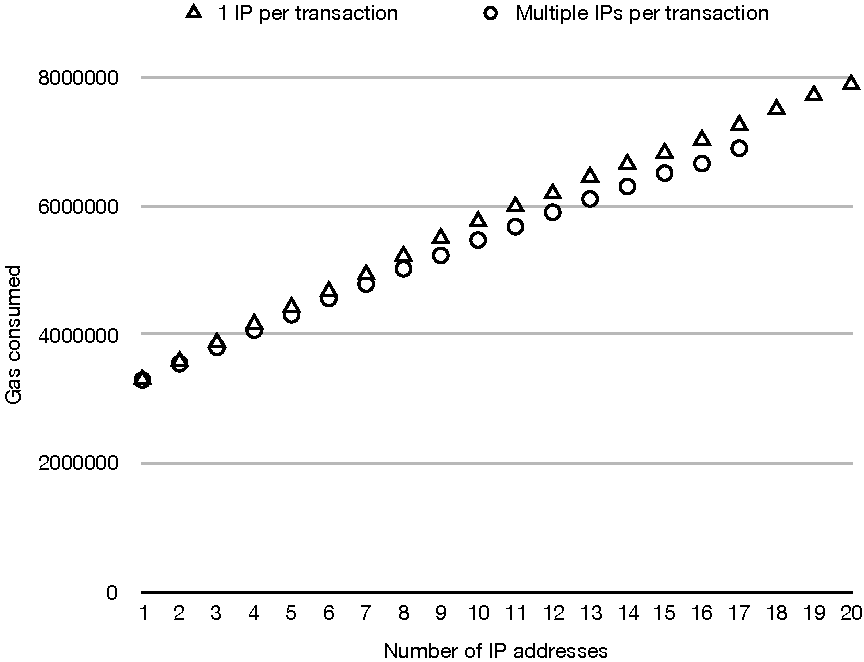
\includegraphics[width=0.7\textwidth]{v3-gas-cost.pdf}
\caption{Gas cost incurred using variant 3}
\label{fig:v3-gas-cost}
\end{figure}

For variant 3 (bloom filter variant), another benchmark script was created\footnote{The source code can be found under \texttt{v3-gas-benchmark.js}. The benchmark can be executed with \texttt{node index v3-gas-benchmark}.}. Like in variant 1, a worst case and a best case scenario was tested, where in the worst case one report gets added at a time, while in the best case, reports could be bundled into one transaction to save gas.

This variant was expected to perform better than variant 1, as less storage is required to store all IP addresses. However, the benchmark does not confirm the expectation. The bloom filter does actually incur more gas costs than storing a full-sized array of IP addresses. 

For adding one report, approximately 290'000 gas is consumed, which is almost three times more than in variant 1 (105'000 gas). There are also no economies of scale, as the cost goes up linearly after the first report. Bundling reports into one transaction does save approximately 40'000 gas per report (13\%), but is less effective than it is for variant 1. Also, it is not possible to add more than 17 reports in one transaction, as the block gas limit is reached.

It becomes clear that Solidity charges more heavily for expensive computation like hashing than it does for storage.
In addition to much higher costs, the bloom filter variant can also give false positives, and metadata like expiration date, whitelist/blacklist etc. has to be stored separately.

If less required storage space does not result in lower prices, then there is no advantage in it at all. The whole blockchain, multiple gigabytes needs to be downloaded to a client anyway \textemdash {} the only reason to optimize for storage is to get cheaper costs.

\chapter{Summary and Conclusions}

Ethereum provides a new platform for decentralized applications of any kind. Using the turing-complete programming language Solidity, smart contracts can be programmed to solve a wide variety of problems.

In order to enable decentralized applications, Ethereum must make some tradeoffs by disincentivizing computation-heavy or space-inefficient applications with cost and limitations.

Several factors decide the cost of Ethereum applications. The complexity of the application, parameters of Ethereum clients and Ether price influence the cost. Speed is correlated to cost with faster transactions for higher prices.

Three protoypes of a smart contract for signaling DDoS attacks for the Ethereum platform were developed, tested and benchmarked. In general, all variants are functional and can be used to store IP addresses. For a small number of IP addresses, the smart contracts are reasonable solutions that are relatively cheap to implement. However, storing more than a few hundred IPs directly in the contract causes serious scalability issues that are hard to overcome on the Ethereum blockchain.

The approach to directly store all IP addresses in an array results in extremely high costs as expected. The supposed solution, the bloom filter, only increased the cost while also introducing imperfect accuracy and eliminating the possibility to obtain a full list of stored IP addresses.

The approach of pointing to a list of IP addresses on the web is the most scalable approach of the three, outsourcing the big data to a established protocol. By testing the integrity of the resources using a hash, the immutability properties of the blockchain can be extended to the web resource as well. On the contrary, this variant is the least ambitious of the solutions and does not fully deliver on the promise of a blockchain-based solution.

In conclusion, Ethereum as a general-purpose blockchain is not the ideal technology to run DDoS signaling applications. However, most of the issues come down to scalability and the developed solutions are viable for signaling small amounts of data. To further advance the idea of decentralized DDoS signaling, specialized blockchains have to be developed which feature properties more suited for this type of application.



\begin{thebibliography}{99}
\addcontentsline{toc}{chapter}{Bibliography}

\bibitem{Ethereum} Ethereum: Blockchain App Platform. \url{https://ethereum.org/}

\bibitem{DDoSRise} Author: Steve Mansfield-Devine. The Growth and Evolution of DDoS. Network
Security 10 (2015), pp. 13-20.

\bibitem{DDoSOverview} Authors: O. Osanaiye, K. Raymond Choo, M. Dlodlo. Distributed denial of service (DDoS) resilience in cloud: Review and conceptual cloud DDoS mitigation framework. 2016 \url{http://www.sciencedirect.com/science/article/pii/S1084804516000023}

\bibitem{DefCOM} Authors: G. Oikonomou, J. Mirkovic, P. Reiher, M. Robinson. A Framework for A Collaborative DDoS Defense. 2006. \url{https://www.acsac.org/2006/papers/123.pdf}

\bibitem{IETFDraft}Authors: K. Nishizuka, L. Xia, J. Xia, D. Zhang, L. Fang, C. Gray, R. Compton. Inter-organization cooperative DDoS protection mechanism \url{https://tools.ietf.org/html/draft-nishizuka-dots-inter-domain-mechanism-02}, Dezember 27, 2016

\bibitem{OriginalPaper} Authors: B. Rodriguez, T. Bocek, A. Lareida, D. Hausheer, S. Rafati, B. Stiller. A Blockchain-based Architecture for Collaborative DDoS Mitigation with Smart Contracts and SDN, 2017

\bibitem{IPv4Exhaustion} RIPE Network Coordination Centre: IPv4 Exhaustion. 2015 \url{https://www.ripe.net/publications/ipv6-info-centre/about-ipv6/ipv4-exhaustion}

\bibitem{EIP74} Author: Alex Beregszaszi. Ethereum Improvement Proposal 74: Support RSA signature verification. \url{https://github.com/ethereum/EIPs/issues/74}

\bibitem{BaselineRequirements} Baseline Requirements Certificate Policy for the Issuance and Management of Publicly-Trusted Certificates \url{https://cabforum.org/wp-content/uploads/CA-Browser-Forum-BR-1.4.5.pdf}

\bibitem{GlobalSign} GlobalSign: Securing a Public IP Address - SSL Certificates
\url{https://support.globalsign.com/customer/portal/articles/1216536-securing-a-public-ip-address---ssl-certificates}

\bibitem{Solc} The Solidity Contract-Oriented Programming Language
\url{https://github.com/ethereum/solidity}


\bibitem{Truffle} Truffle Framework \url{http://truffleframework.com/}

\bibitem{Solium} Solium Framework \url{https://github.com/duaraghav8/Solium}

\bibitem{ThinkingAboutSmartContractSecurity} Autor: V. Buterin, \url{https://blog.ethereum.org/2016/06/19/thinking-smart-contract-security}, 19. Juni 2016.


\bibitem{EIP150} Author: Vitalik Buterin. Ethereum Improvement Proposal 150: Long-term gas cost changes for IO-heavy operations to mitigate transaction spam attacks. \url{https://github.com/ethereum/EIPs/issues/150}


\bibitem{DefaultGoEthereumConfiguration} go-ethereum Github Repository. File \texttt{eth/config.go}. \url{https://github.com/ethereum/go-ethereum/blob/fff16169c64a83d57d2eed35b6a2e33248c7d5eb/eth/config.go\#L45}

\bibitem{ETHGasStationAnnouncement} Author: @ethgasstation. The Safe Low Gas Price \url{https://medium.com/@ethgasstation/the-safe-low-gas-price-fb44fdc85b91}



\end{thebibliography}



\chapter*{Abbreviations}
\addcontentsline{toc}{chapter}{Abbreviations}
\markboth{ABBREVIATONS}{}


\abr{ABI}{Application Binary Interface}
\abr{CA}{Certificate Authority}
\abr{CDN}{Content Distribution Network}
\abr{CSV}{Comma separated values}
\abr{DoS}{Denial of Service}
\abr{DDoS}{Distributed Denial of Service}
\abr{ETH}{Ether (currency of Ethereum)}
\abr{FNV}{Fowler-Noll-Vo}
\abr{HTTP}{Hypertext Transfer Protocol}
\abr{HTTPS}{Hypertext Transfer Protocol Secure}
\abr{IP}{Internet Protocol}
\abr{IPv4}{Internet Protocol Version 4}
\abr{IPv6}{Internet Protocol Version 6}
\abr{ISP}{Internet Service Provider}
\abr{JSON}{Javascript Object Notation}
\abr{npm}{Node package manager}
\abr{REST}{Representational State Transfer}
\abr{SHA}{Secure Hash algorithm}
\abr{solc}{Solidity compiler}
\abr{URL}{Uniform Resource Locator}
\abr{XML}{Extensible Markup Language}

\chapter*{Glossary}
\addcontentsline{toc}{chapter}{Glossary}
\markboth{GLOSSARY}{}


\begin{description}
  \item[Authentication] 
  \item[Authorization] Authorization is the decision whether an entity is allowed to perform a particular action or not, 
       e.g. whether a user is allowed to attach to a network or not.
  \item[Accounting]
\end{description}


\addcontentsline{toc}{chapter}{List of Figures}
\listoffigures
%\addcontentsline{toc}{chapter}{List of Tables}
%\listoftables

%\appendix

\chapter{Installation Guidelines}

\chapter{Contents of the CD}


\textbf{code/}: The source code of the project.

\textbf{Raw data.xls}: Excel spreadsheet containing all the raw data and calculations needed to create the figures.

\textbf{Related Work/}: A collection of related work papers.

\textbf{tex/}: The source code for this document.


\end{document}
